\documentclass[11pt,a4paper]{article}

\usepackage[utf8]{inputenc}
\usepackage[T1]{fontenc}
\usepackage[margin=2.5cm]{geometry}
\usepackage{graphicx}
\usepackage{booktabs}
\usepackage{longtable}
\usepackage{xcolor}
\usepackage{enumitem}
\usepackage{titlesec}
\usepackage{caption}
\usepackage{hyperref}
\usepackage{amsmath}
\usepackage{amssymb}
\setlength{\emergencystretch}{3em}
\sloppy

\graphicspath{{figs/}}

\definecolor{accentblue}{HTML}{2E5395}
\titleformat{\section}{\Large\bfseries\color{accentblue}}{\thesection}{0.5em}{}
\titleformat{\subsection}{\large\bfseries\color{accentblue}}{\thesubsection}{0.5em}{}
\titleformat{\subsubsection}{\normalsize\bfseries\color{accentblue}}{\thesubsubsection}{0.5em}{}

\captionsetup{font={small,it,color=black!60},labelfont={bf,it}}

\hypersetup{colorlinks=true, linkcolor=accentblue, urlcolor=accentblue}

\setlist[itemize]{leftmargin=1.4em, itemsep=3pt, topsep=3pt}

\title{\vspace{-1.5cm}{\color{accentblue}\textbf{FastSDPCertification}}\\[4pt]
\textbf{\Large Experiment Summary --- McCormick ``composed'' vs baseline on cross-product terms}\\[4pt]
{\normalsize\itshape\color{black!60} Network blob\_nn\_4x10-1 --- 330 cross-product terms tested individually}}
\author{}
\date{}

\begin{document}
\maketitle
\vspace{-1.3cm}

\section{Objective}
In the SDP relaxation used to certify the \texttt{blob\_nn\_4x10-1} network, every cross-product term of two neurons $z_{l,u} \cdot z_{k,j}$ can be relaxed in two ways: the baseline strategy (\texttt{one\_variable}, also called \texttt{none}/\texttt{simple} in the files), or a finer but more expensive McCormick relaxation, \texttt{composed}. The experiment aims to determine, term by term, whether switching to \texttt{composed} actually improves the certification rate and the optimal value of the SDP program, and whether this choice can be predicted automatically from the bounds (LB/UB) of the two neurons involved, without having to test every single term with the solver. This report walks through the analysis in the order it was actually done: first at the level of per-combo means, then at the level of individual data points, then with a trained decision tree --- and ends on why, in practice, \texttt{one\_variable} everywhere turns out to be the most defensible default.

\section{Methodology}
\begin{itemize}
  \item \textbf{Baseline} (\texttt{combo\_0000}): all 330 cross-product terms of the network are set to \texttt{one\_variable}.
  \item \textbf{330 test combos}: each \texttt{combo\_XXXX} starts from the baseline and flips exactly one term (layer $l$, neuron \texttt{u\_idx}) $\times$ (layer $k$, neuron \texttt{j\_idx}) to \texttt{composed}.
  \item Each combo is evaluated on a test set of 78 to 80 data points; for every point we record \texttt{certified} (\texttt{optimal\_value > 0}), \texttt{optimal\_value}, and the \texttt{gain} relative to the baseline on that same point. \textbf{Definition:} $\texttt{gain} = \texttt{optimal\_value}_{\text{combo}} - \texttt{optimal\_value}_{\text{baseline}}$, computed point by point (same \texttt{data\_index}, same combo's own bounds vs.\ the baseline's optimal value on that exact point) --- so \texttt{gain} isolates the effect of switching this one term to \texttt{composed}, independently of how easy or hard that particular test point is to certify in the first place.
  \item \textbf{Computational cost.} Every one of these solves goes through MOSEK, and MOSEK is genuinely slow at this scale: the project's cumulative \texttt{Mosek\_logger.log} has grown to \textbf{2.8\,GB} and records \textbf{14{,}608 individual solver calls} spread over roughly \textbf{two months} of intermittent runs (9~June -- 11~August 2026) across the project's various experiments. Each single MOSEK call is quick on its own (typically 0.03--0.1\,s, per the log), but with 330 candidate terms $\times$ 78--80 test points, a single full pass of this experiment requires tens of thousands of separate solves --- that per-call overhead and queueing, not the solver's raw speed, is what makes a full combo sweep take hours to run in practice. This is precisely the motivation for trying to replace solver calls with a lightweight predictor: it would remove the need to re-run MOSEK for every candidate term.
\end{itemize}

\section{First pass: working with the mean of each combo}
The first analysis pass collapsed every combo down to a single row: the mean \texttt{optimal\_value}/\texttt{gain} over its test points, and the mean LB/UB bounds of its two neurons over that same test set. This section presents that pass in full, then explains why its results were not very conclusive.

\subsection{Aggregate comparison: composed vs baseline}
Across the 130 successfully tested combos (with 3 baseline runs kept as reference), \texttt{composed} brings, on average, no net benefit:

\begin{center}
\begin{tabular}{lcc}
\toprule
\textbf{Strategy} & \textbf{Mean certification rate} & \textbf{Mean optimal value} \\
\midrule
Baseline (\texttt{none}) & 50.9\% & $-3.03$ \\
Composed (average of 130 combos) & 49.9\% & $-3.18$ \\
\bottomrule
\end{tabular}
\end{center}

\clearpage

\subsection{Separating combos by their mean optimal value (\texttt{separation\_plot.ipynb})}
\texttt{separation\_plot.ipynb} looks inside the 130 composed rows: it trains a depth-4 decision tree (\texttt{min\_samples\_leaf=3}) on \texttt{l, u\_idx, k, j\_idx, LB\_neuron1, UB\_neuron1, LB\_neuron2, UB\_neuron2} (all of them \textbf{means over the test set}) to predict \texttt{optimal\_value\_avg}, ranks the features by importance, and plots the tree's predicted surface over its top-2 features with a ``composed cutoff'' line at $\text{mean}+1\,\sigma$ of the predicted values.

Re-running this exact pipeline gives \texttt{UB\_neuron2} (importance $0.605$) and \texttt{u\_idx} ($0.388$) as by far the two most important features --- \texttt{l}, \texttt{k}, \texttt{j\_idx} score $0.000$. Over the 130 composed combos, \texttt{optimal\_value\_avg} ranges from $-3.203$ to $-2.731$ (mean $-3.179$, std $0.056$), and the cutoff line sits at $-3.150$.

\begin{figure}[h!]
  \centering
  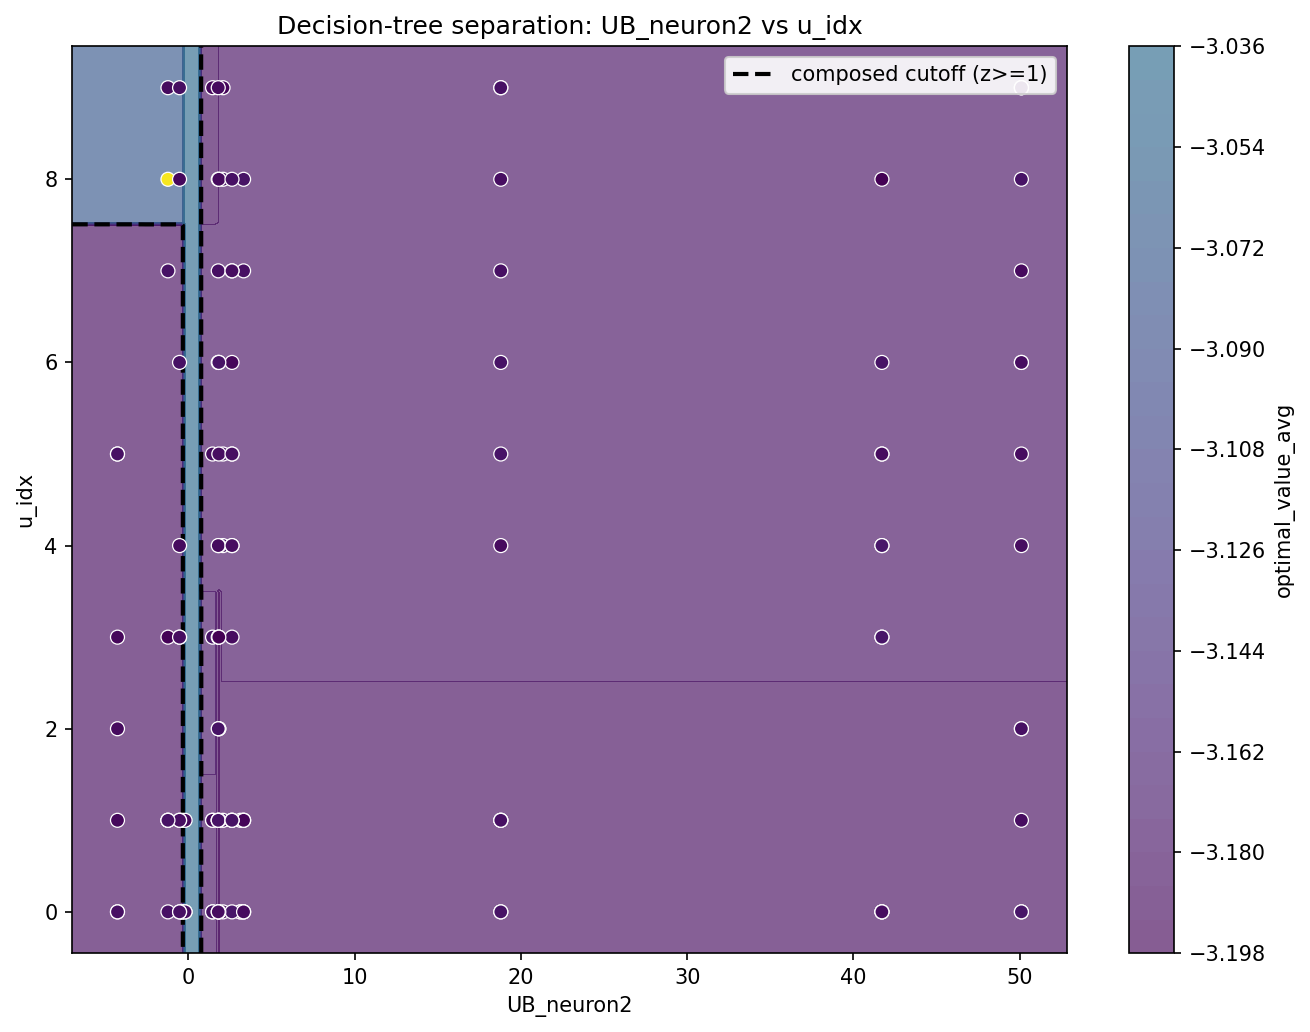
\includegraphics[width=0.68\textwidth]{separation_plot_verified.png}
  \caption{\texttt{separation\_plot.ipynb} output: \texttt{UB\_neuron2} vs.\ \texttt{u\_idx} (mean bounds), coloured by \texttt{optimal\_value\_avg}. The background is almost uniformly the same shade ($\approx -3.15$ to $-3.20$) except for a thin vertical band near $\text{UB\_neuron2}\approx 0$.}
  \label{fig:separation}
\end{figure}

\begin{figure}[h!]
  \centering
  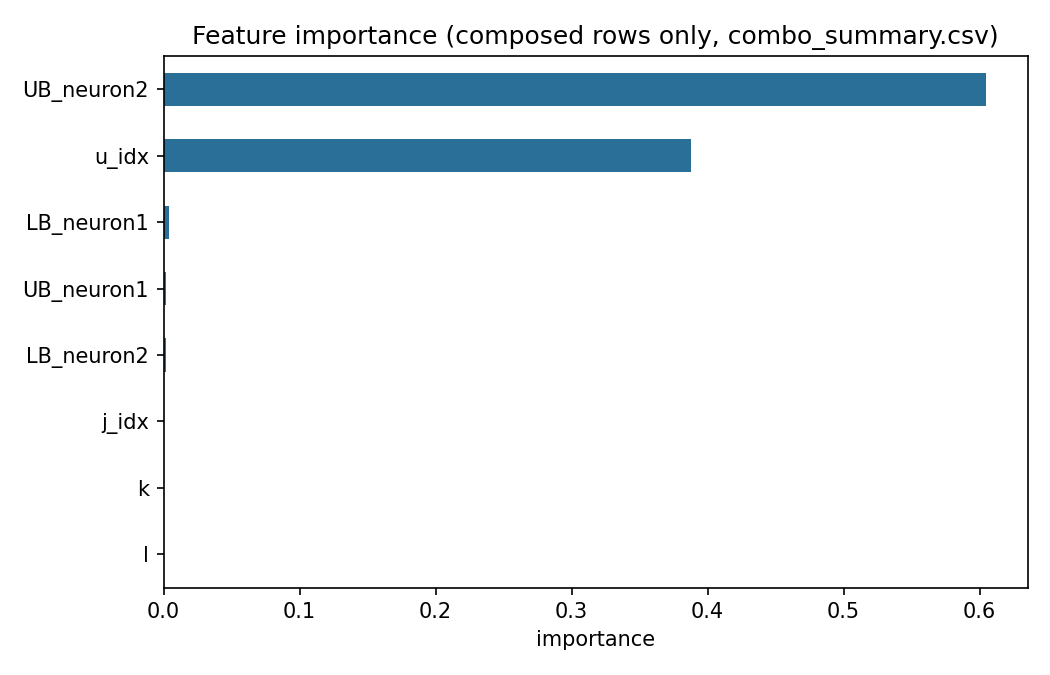
\includegraphics[width=0.6\textwidth]{feature_importance_verified.png}
  \caption{Feature importance of that tree (130 composed rows): \texttt{UB\_neuron2} and \texttt{u\_idx} carry essentially all of it; \texttt{l}, \texttt{k}, \texttt{j\_idx} contribute exactly $0$.}
  \label{fig:featimp}
\end{figure}

\clearpage

\subsection{Distribution of the mean gain per combo}
The mean gain (composed $-$ baseline) per combo is almost always close to zero, and slightly negative for the majority of combos: out of 158 aggregated combos, 92 have a negative or zero mean gain.

\begin{figure}[h!]
  \centering
  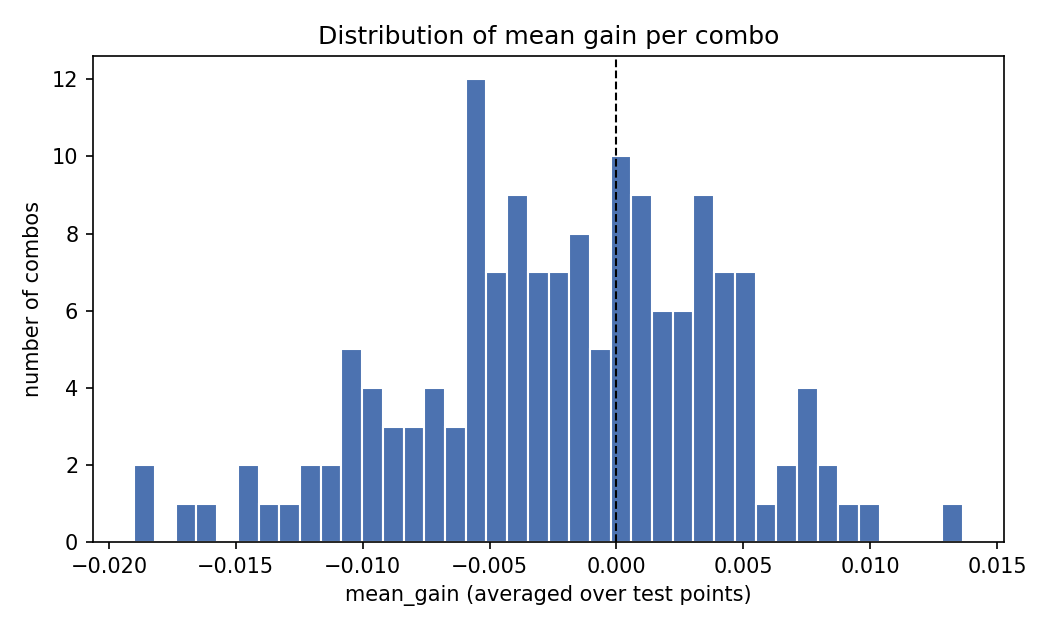
\includegraphics[width=0.68\textwidth]{A_distribution_gain_par_combo.png}
  \caption{Distribution of the mean gain per combo.}
  \label{fig:gaindist}
\end{figure}

\subsection{Applying the (later) tree rules to per-combo means}
As a sanity check, the fixed rules of the trained gain-regression tree from Section~\ref{sec:tree} were applied to these same per-combo \textbf{mean} bounds instead of per-point bounds (\texttt{classify\_combos\_from\_runs.py}, output \texttt{combo\_classification.csv}). Result: \textbf{309 out of 309} evaluated combos get a predicted gain of exactly $0.00$ and are labelled \texttt{simple} (\texttt{one\_variable}) --- not one single combo's mean bounds fall inside the narrow window that the tree associates with a positive gain.

\subsection{Interpretation: not very conclusive, and the bounds are not rigorously defined}
Two things stand out from this first pass:
\begin{itemize}
  \item \textbf{The results are not very conclusive.} The separation found (Fig.~\ref{fig:separation}) is real but narrow, the aggregate composed/baseline comparison shows no net benefit, and applying the eventual tree rule to these same per-combo figures recommends \texttt{one\_variable} for literally every combo (Section~3.4). Nothing here points decisively towards \texttt{composed} being worth it anywhere.
  \item \textbf{``The bounds are the most important feature'' is not a rigorous statement at this level.} \texttt{UB\_neuron2} tops the feature-importance ranking (Fig.~\ref{fig:featimp}), but what is actually being ranked is the \textbf{mean} of \texttt{UB\_neuron2} over 78--80 test points --- a quantity the solver never sees directly (it only ever sees one point's exact bound at a time). Why average at all, rather than, say, using the tightest or widest bound actually reached across the test set? Nothing in this pipeline justifies the mean specifically over any other summary statistic, so ``the bounds matter'' is true only in a loose sense here: it tells us bounds are \emph{worth looking at}, not that this particular (mean) definition of them is the right one to act on.
\end{itemize}
This is what motivated moving to the per-data-point analysis below, where ``the bounds'' finally have an unambiguous meaning: the exact \texttt{LB}/\texttt{UB} of the two neurons, for that one specific test point.

\clearpage

\section{Second pass: using every single data point}
This reproduces the pipeline of the \texttt{combo\_visualisation.ipynb} notebook (Section~7), run directly on \texttt{combo\_detail\_by\_datapoint.csv} (18{,}018 usable rows after cleaning, one row per test point per combo --- no averaging, so \texttt{LB\_neuron1, UB\_neuron1, LB\_neuron2, UB\_neuron2} are now each point's own exact bounds). A depth-3 regression tree is trained, with a 75/25 train/test split (\texttt{random\_state=0}), to predict the continuous \texttt{gain}.

\subsection{Gain regression}
The tree trained on \texttt{LB\_neuron1, UB\_neuron1, LB\_neuron2, UB\_neuron2} achieves an $R^2$ of \textbf{0.027 on the test set} (0.029 on train): it does capture a real spread between leaves ($-0.09$ to $+0.23$), but only explains $\approx 3\%$ of the variance in gain --- most of the point-by-point noise is left unexplained. Adding \texttt{k, l} changes nothing (test $R^2 = 0.026$).

\begin{figure}[h!]
  \centering
  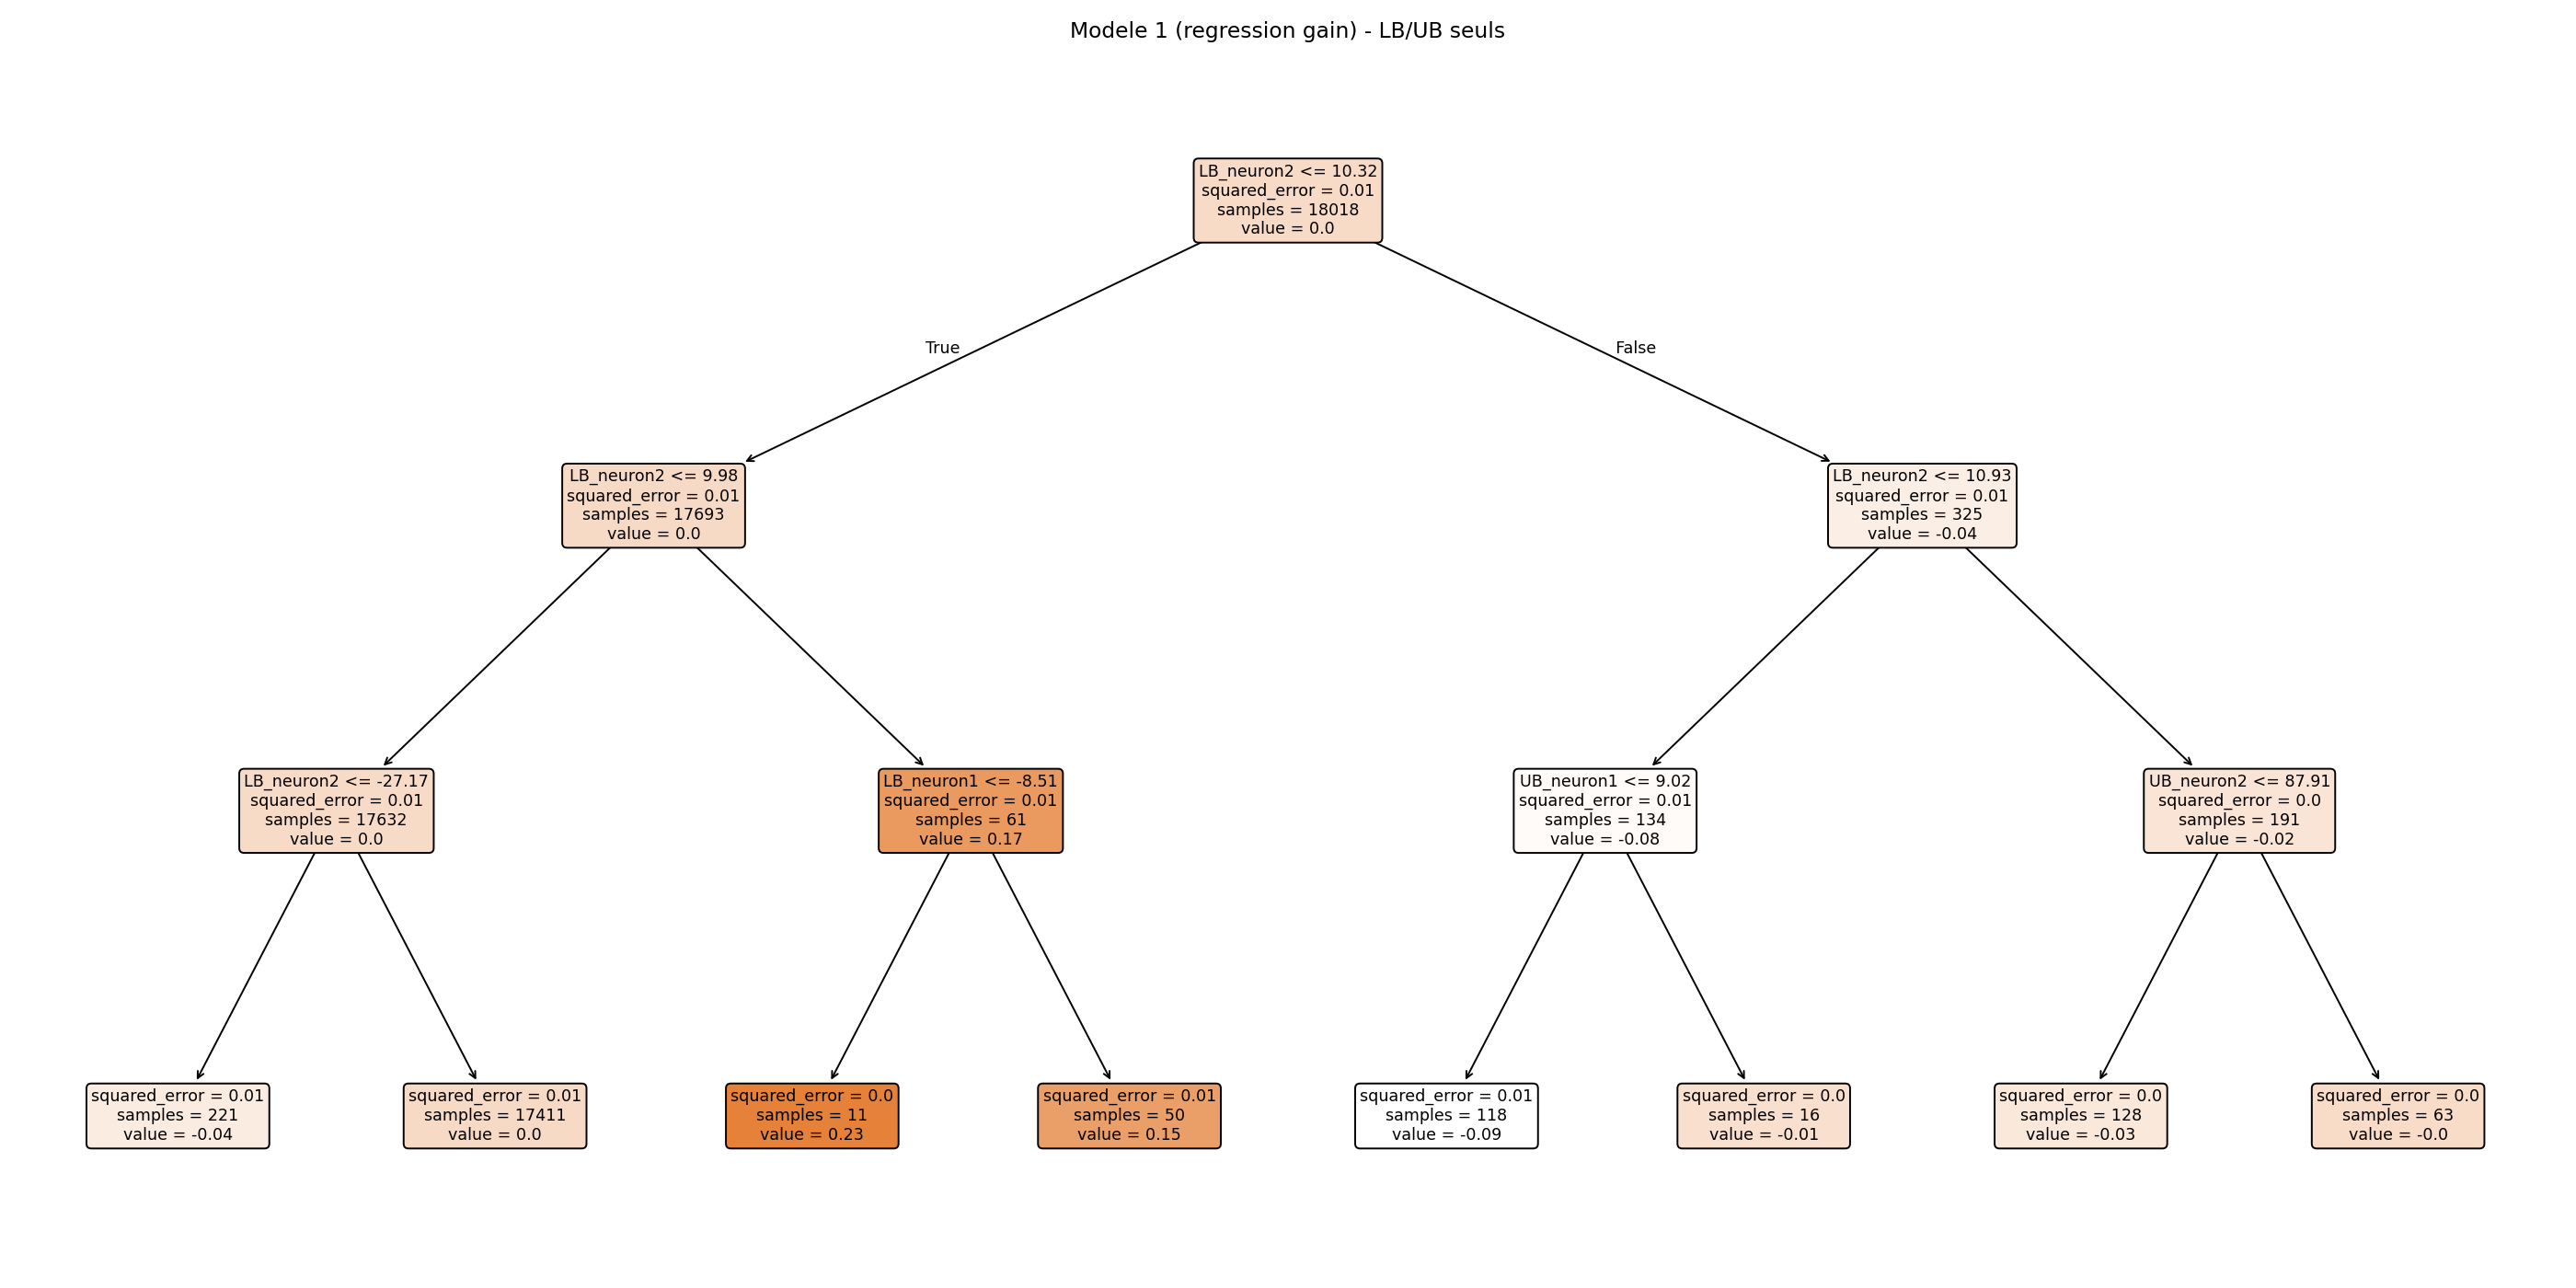
\includegraphics[width=\textwidth]{7a_tree_reg_bounds.png}
  \caption{Regression tree (gain), depth 3, on the per-point \texttt{LB\_neuron1, UB\_neuron1, LB\_neuron2, UB\_neuron2}. Test $R^2 = 0.027$.}
  \label{fig:regtree}
\end{figure}

\clearpage

\subsection{Interpretation}
Using every single data point instead of per-combo means resolves the ambiguity from Section~3: the bounds here are exact, not averaged, so a feature-importance ranking on them is a statement about actual solver inputs. Even so, the gain model (Fig.~\ref{fig:regtree}), which is the one that actually decides \texttt{composed} vs \texttt{one\_variable}, stays weak ($R^2 \approx 0.03$) --- moving from combo-level means to exact, per-point bounds removed the definitional ambiguity from Section~3, but it did not turn this into a strong predictor of gain.

\clearpage

\section{The trained tree, and where the gain drops away}
\label{sec:tree}
The gain-regression tree from Section~4.1 is the model actually used to decide \texttt{composed} vs \texttt{one\_variable} per term. Its rules:

\begin{center}
\begin{tabular}{lcc}
\toprule
\textbf{Rule (learned thresholds, gain model)} & \textbf{Samples} & \textbf{Predicted gain} \\
\midrule
$\text{LB\_neuron2} \le -27.17$ & $221$ & $-0.040$ \\
$-27.17 < \text{LB\_neuron2} \le 9.98$ & $17{,}411$ & $+0.004$ \\
$9.98 < \text{LB\_neuron2} \le 10.32$ \;and\; $\text{LB\_neuron1} \le -8.51$ & $11$ & $+0.229$ \\
$9.98 < \text{LB\_neuron2} \le 10.32$ \;and\; $\text{LB\_neuron1} > -8.51$ & $50$ & $+0.161$ \\
$10.32 < \text{LB\_neuron2} \le 10.93$ \;and\; $\text{UB\_neuron1} \le 9.02$ & $118$ & $-0.089$ \\
$10.32 < \text{LB\_neuron2} \le 10.93$ \;and\; $\text{UB\_neuron1} > 9.02$ & $16$ & $-0.011$ \\
$\text{LB\_neuron2} > 10.93$ \;and\; $\text{UB\_neuron2} \le 87.91$ & $128$ & $-0.032$ \\
$\text{LB\_neuron2} > 10.93$ \;and\; $\text{UB\_neuron2} > 87.91$ & $63$ & $-0.001$ \\
\bottomrule
\end{tabular}
\end{center}

Only two of these eight leaves are positive, and they both require \texttt{LB\_neuron2} to sit inside a window barely $0.34$ wide ($9.98$ to $10.32$); every other leaf --- covering the rest of the real line --- is at or below zero. The \textbf{samples} column makes the imbalance concrete: the two positive leaves together hold only $11+50=61$ of the $18{,}018$ training points ($0.34\%$), while the single largest leaf ($-27.17 < \text{LB\_neuron2}\le 9.98$, $17{,}411$ points, $96.6\%$ of the data) predicts an essentially-zero gain of $+0.004$. This is the ``drop in gain'' visible at every level of this report:
\begin{itemize}
  \item at the raw per-point level, the best a single leaf ever predicts is $+0.229$ (on just $11$ points), next to leaves as low as $-0.089$ (on $118$ points);
  \item once bounds are averaged per combo instead of taken per point (Section~3.4), the gain drops to exactly $0.00$ for \textbf{all 309} combos checked --- the narrow positive window essentially never survives averaging, because it is $0.34$ wide against a range of tens of units.
\end{itemize}
The specific, narrow condition under which \texttt{composed} is predicted to actually help essentially never holds once you can no longer cherry-pick a single favourable data point in advance.

\section{Validating the tree on a real run (\texttt{compare\_runs.ipynb})}
\label{sec:comparerun}
Everything up to this point was cross-validation on historical solver data. \texttt{compare\_runs.ipynb} instead runs the actual pipeline with \texttt{relu\_relaxation\_type: "auto"} --- meaning the trained gain-tree from Section~\ref{sec:tree} decides \texttt{composed} vs \texttt{one\_variable} live, term by term, from each point's own bounds --- and compares its solver output directly against a \texttt{one\_variable}-everywhere baseline, point by point.

\subsection{Setup}
\begin{itemize}
  \item \textbf{Comparison run:} \texttt{relu\_relaxation\_type: "auto"}, executed 2026-08-11 on \texttt{blob\_nn\_4x10-1} over a 1000-image batch (872 points actually recorded, in five parts).
  \item \textbf{Baseline:} two available \texttt{combo\_0000} (all-\texttt{one\_variable}) runs, both from 2026-08-07, each with 80 points (\texttt{data\_index} 0--79).
  \item \textbf{Matching:} following \texttt{compare\_runs.ipynb} exactly, both sides are sorted by \texttt{data\_index} and truncated to the first 78 points (the same test-set size used everywhere else in this report). All 78 \texttt{data\_index} values coincide exactly between baseline and comparison (same 78 images), so this is a genuine point-by-point comparison, not a positional guess.
\end{itemize}

\subsection{Results}
Using the first baseline run as the reference:

\begin{center}
\begin{tabular}{lc}
\toprule
\textbf{Quantity} & \textbf{Value} \\
\midrule
Matched points & 78 \\
Mean gain (auto $-$ baseline) & $-0.178$ \\
Median gain & $-0.116$ \\
Points with gain $>0$ & $4$ ($5.1\%$) \\
Points with gain $<0$ & $73$ ($94.9\%$) \\
Largest positive gain & $+3.7\times10^{-7}$ \\
Most negative gain & $-0.804$ \\
Newly certified (baseline no $\to$ auto yes) & $0$ \\
Newly lost (baseline yes $\to$ auto no) & $4$ \\
Certification rate, baseline & $52.6\%$ \\
Certification rate, auto (tree) & $47.4\%$ \\
\bottomrule
\end{tabular}
\end{center}

\begin{figure}[h!]
  \centering
  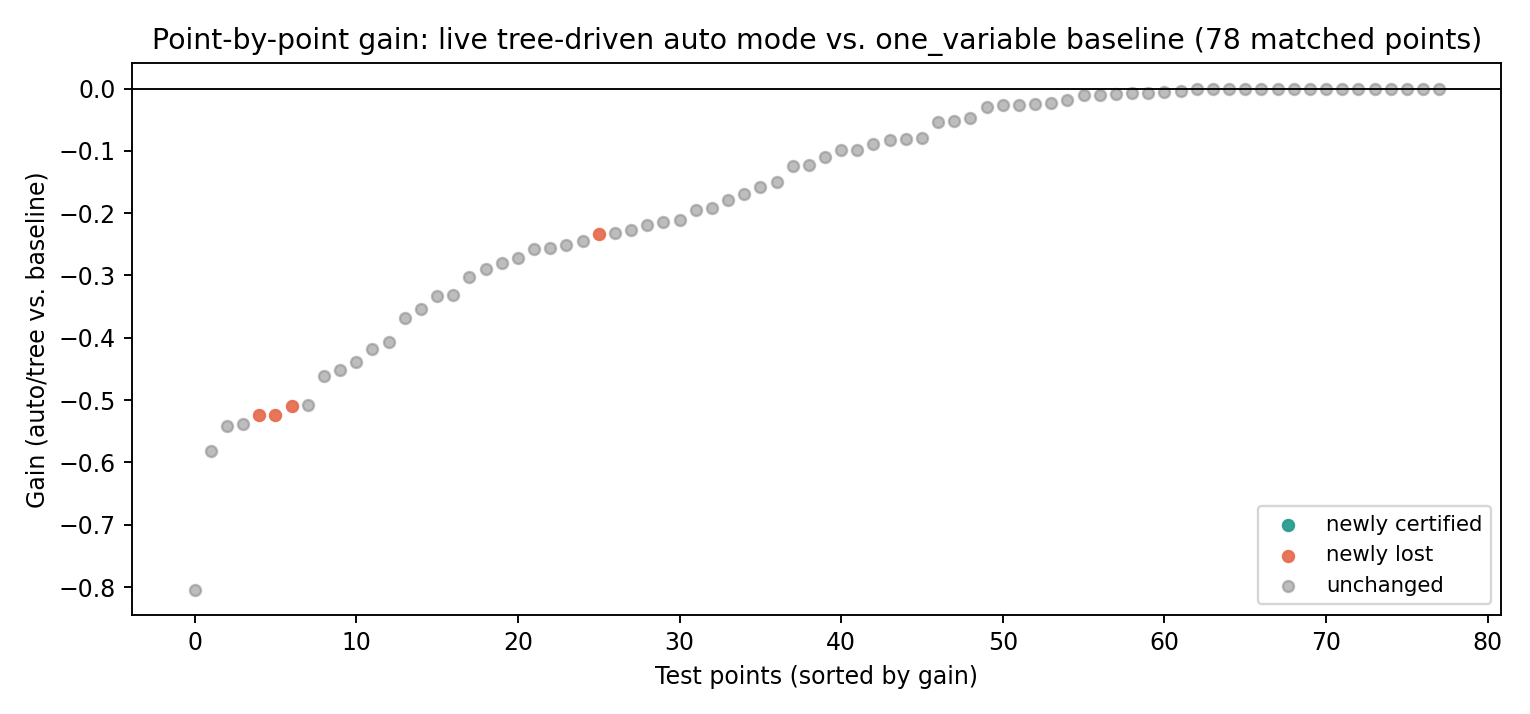
\includegraphics[width=0.85\textwidth]{C_compare_runs_auto_vs_baseline.png}
  \caption{Point-by-point gain of the live, tree-driven \texttt{auto} mode relative to the \texttt{one\_variable} baseline, on the 78 matched test points. Almost every point is at or below zero; the few points shown above zero are of order $10^{-7}$--$10^{-8}$ (solver noise, not a real gain).}
  \label{fig:comparerun}
\end{figure}

The four points with a nominally positive gain are all of order $10^{-7}$ to $10^{-8}$ --- far below anything that could be called a real improvement. Re-running the same comparison against the \emph{second} available baseline run gives the same picture (mean gain $-0.179$, certification rate $52.6\%\to47.4\%$, the same 4 points newly lost and 0 newly gained); the one point that looked nominally positive against that second baseline ($+0.031$) is smaller than the $\approx 0.33$ run-to-run variation MOSEK itself produces between the two baseline runs on that exact same image, so it cannot be distinguished from ordinary solver noise either.

\subsection{Interpretation}
This is the one part of the analysis that is not cross-validation or leaf statistics: it is the trained tree actually driving solver decisions on a real, previously-unseen batch of 872 images, compared point by point against always using \texttt{one\_variable}. The result matches every earlier warning sign in this report --- the mean gain is clearly negative, the certification rate drops by 5.2 points, and not a single point shows a gain large enough to distinguish from solver noise. Letting the tree decide live does not merely fail to help; on this run it makes both the optimal value and the certification rate worse than the \texttt{one\_variable} baseline.

\section{Conclusions}
\begin{itemize}
  \item \textbf{First pass (per-combo means, Section~3):} not conclusive --- \texttt{composed} shows no net benefit on average, and the ``important'' bounds identified there are means over the test set, a quantity with no clear operational meaning (the solver never sees a mean bound). This motivated moving to per-point data.
  \item \textbf{Second pass (per data point, Section~4):} with bounds unambiguously defined, exactly rather than averaged, the \textbf{gain} model --- the one that actually drives the \texttt{composed} decision --- still stays weak ($R^2\approx 0.03$).
  \item \textbf{The trained tree (Section~\ref{sec:tree}):} only a $0.34$-wide window of \texttt{LB\_neuron2} predicts a positive gain; everywhere else is at or below zero, and that window does not survive averaging bounds per combo (0 of 309 combos recommended \texttt{composed} when checked that way).
  \item \textbf{Validating the tree on a real run (Section~\ref{sec:comparerun}):} letting the tree decide \texttt{composed} vs \texttt{one\_variable} live, point by point, on a real 78-point held-out batch makes things worse, not better --- mean gain $-0.178$, certification rate down from $52.6\%$ to $47.4\%$, and not one point shows a gain that rises above solver noise. This is not an extrapolation from cross-validated statistics: it is the tree's own live decisions performing worse than the fixed \texttt{one\_variable} baseline.
  \item \textbf{MOSEK is already the practical bottleneck} (Section~2): 14{,}608 individual solves and 2.8\,GB of logs accumulated on this project. Chasing a narrow, unreliable gain window is not worth the additional solver calls it would cost to validate per term.
  \item \textbf{Conclusion:} given that (a) \texttt{composed} shows no benefit on average, (b) its gain model is weak and its one favourable region is a sliver that disappears under any reasonable aggregation, and (c) letting the tree drive decisions live on a real run actually reduced the certification rate, using \texttt{one\_variable} for every single cross-product term is the most reasonable, defensible default --- at least until a dedicated experiment demonstrates a targeted \texttt{composed} choice that actually holds up.
  \item \textbf{Limitation}: the tree and its thresholds were learned on a single network (\texttt{blob\_nn\_4x10-1}) and a single test set; their generalization to other architectures or datasets still needs to be checked. In practice, this is largely a consequence of MOSEK's own runtime: at 14{,}608 solves and 2.8\,GB of logs already spent on this one network (Section~2), repeating the same combo-by-combo sweep on larger or additional networks was not feasible within the time available for this experiment.
\end{itemize}

\vspace{1em}
{\small\itshape\color{black!55} Sources: \texttt{scripts/combo\_summary.csv}, \texttt{combo\_summary\_aggregated.csv}, \texttt{combo\_classification.csv}, \texttt{combo\_detail\_by\_datapoint.csv}, \texttt{separation\_plot.ipynb}, \texttt{classify\_combos\_from\_runs.py}, \texttt{bound\_type\_predictor.py}, \texttt{compare\_runs.ipynb}, \texttt{results/benchmark/blob\_nn\_4x10-1/2026\_08\_11\_00h46\_41s\_/} (auto/tree run), \texttt{results/benchmark/blob\_nn\_4x10-1/loop\_705\_combo\_0000\_\_baseline\_\_all\_one\_variable/} and \texttt{loop\_873\_...} (baseline runs), \texttt{results/Mosek\_logger.log} --- \texttt{scripts/} and \texttt{results/} folders of the FastSDPCertification project.}

\end{document}
